%%%%%%%%%%%%%%%%%%%%%%%%%%%%%%%%%%%%%%%%%
% Short Sectioned Assignment LaTeX Template Version 1.0 (5/5/12)
% This template has been downloaded from: http://www.LaTeXTemplates.com
% Original author:  Frits Wenneker (http://www.howtotex.com)
% License: CC BY-NC-SA 3.0 (http://creativecommons.org/licenses/by-nc-sa/3.0/)
%%%%%%%%%%%%%%%%%%%%%%%%%%%%%%%%%%%%%%%%%

% \documentclass[paper=a4, fontsize=11pt]{scrartcl} % A4 paper and 11pt font size
\documentclass[11pt, a4paper]{book}
\usepackage[T1]{fontenc} % Use 8-bit encoding that has 256 glyphs
\usepackage[utf8]{inputenc}
\usepackage{fourier} % Use the Adobe Utopia font for the document - comment this line to return to the LaTeX default
\usepackage{listings} % para insertar código con formato similar al editor
\usepackage[spanish, es-tabla]{babel} % Selecciona el español para palabras introducidas automáticamente, p.ej. "septiembre" en la fecha y especifica que se use la palabra Tabla en vez de Cuadro
\usepackage{url} % ,href} %para incluir URLs e hipervínculos dentro del texto (aunque hay que instalar href)
\usepackage{graphics,graphicx, float} %para incluir imágenes y colocarlas
\usepackage[gen]{eurosym} %para incluir el símbolo del euro
\usepackage{cite} %para incluir citas del archivo <nombre>.bib
\usepackage{enumerate}
\usepackage{hyperref}
\usepackage{graphicx}
\usepackage{tabularx}
\usepackage{booktabs}

\usepackage[table,xcdraw]{xcolor}
\hypersetup{
	colorlinks=true,	% false: boxed links; true: colored links
	linkcolor=black,	% color of internal links
	urlcolor=cyan		% color of external links
}
\renewcommand{\familydefault}{\sfdefault}
\usepackage{fancyhdr} % Custom headers and footers
\pagestyle{fancyplain} % Makes all pages in the document conform to the custom headers and footers
\fancyhead[L]{} % Empty left header
\fancyhead[C]{} % Empty center header
\fancyhead[R]{Sergio Cervilla Ortega} % My name
\fancyfoot[L]{} % Empty left footer
\fancyfoot[C]{} % Empty center footer
\fancyfoot[R]{\thepage} % Page numbering for right footer
%\renewcommand{\headrulewidth}{0pt} % Remove header underlines
\renewcommand{\footrulewidth}{0pt} % Remove footer underlines
\setlength{\headheight}{13.6pt} % Customize the height of the header

\usepackage{titlesec, blindtext, color}
\definecolor{gray75}{gray}{0.75}
\newcommand{\hsp}{\hspace{20pt}}
\titleformat{\chapter}[hang]{\Huge\bfseries}{\thechapter\hsp\textcolor{gray75}{|}\hsp}{0pt}{\Huge\bfseries}
\setcounter{secnumdepth}{4}

\begin{document}

	% Plantilla portada UGR
	\begin{titlepage}
\newlength{\centeroffset}
\setlength{\centeroffset}{-0.5\oddsidemargin}
\addtolength{\centeroffset}{0.5\evensidemargin}
\thispagestyle{empty}

\noindent\hspace*{\centeroffset}\begin{minipage}{\textwidth}

\centering

\includegraphics[width=0.9\textwidth]{imagenes/logo_ugr.jpg}\\[1.4cm]

\textsc{ \Large TRABAJO FIN DE GRADO\\[0.2cm]}
\textsc{ GRADO EN INGENIERIA INFORMATICA}\\[1cm]

{\Huge\bfseries Chief \\}
\noindent\rule[-1ex]{\textwidth}{3pt}\\[3.5ex]
{\large\bfseries Apoyo a la labor de la Policía Local }
\end{minipage}

\vspace{2.5cm}
\noindent\hspace*{\centeroffset}
\begin{minipage}{\textwidth}
\centering

\textbf{Autor}\\ {Sergio Cervilla Ortega}\\[2.5ex]
\textbf{Director}\\ {Juan Julián Merelo Guervós}\\[2cm]

\includegraphics[width=0.3\textwidth]{imagenes/etsiit_logo.png}\\[0.1cm]
\textsc{Escuela Técnica Superior de Ingenierías Informática y de Telecomunicación}\\
\textsc{---}\\
Granada, algún mes de 2018
\end{minipage}
\end{titlepage}

	
	% Plantilla prefacio UGR
	\chapter*{}
\thispagestyle{empty}

\begin{center}
{\large\bfseries Chief \\ Apoyo a la labor de la Policía Local}\\
\end{center}
\begin{center}
Sergio Cervilla Ortega\\
\end{center}

%\vspace{0.7cm}

\noindent{\textbf{Resumen}}\\

Lorem ipsum dolor sit amet, consectetur adipisicing elit, sed do eiusmod tempor incididunt ut labore et dolore magna aliqua. Ut enim ad minim veniam, quis nostrud exercitation ullamco laboris nisi ut aliquip ex ea commodo consequat. Duis aute irure dolor in reprehenderit in voluptate velit esse cillum dolore eu fugiat nulla pariatur. Excepteur sint occaecat cupidatat non proident, sunt in culpa qui officia deserunt mollit anim id est laborum.

\cleardoublepage

\thispagestyle{empty}

\noindent\rule[-1ex]{\textwidth}{2pt}\\[4.5ex]

D. \textbf{Juan Julián Merelo Guervós}, Profesor del Área de XXXX del Departamento de Arquitectura y Tecnología de Computadores de la Universidad de Granada.

\vspace{0.5cm}

\textbf{Informo:}

\vspace{0.5cm}

Que el presente trabajo, titulado \textit{\textbf{Chief, blah blah}},
ha sido realizado bajo mi supervisión por \textbf{Sergio Cervilla Ortega}, y autorizo la defensa de dicho trabajo ante el tribunal
que corresponda.

\vspace{0.5cm}

Y para que conste, expiden y firman el presente informe en Granada a X de mes de 2018.

\vspace{1cm}

\textbf{El director: }

\vspace{5cm}

\noindent \textbf{Juan Julián Merelo Guervós}

	
	% Índice de contenidos
	\newpage
	\tableofcontents

	% Índice de imágenes y tablas
	\newpage
	\listoffigures

	% Si hay suficientes se incluirá dicho índice
	\listoftables 
	\newpage
	

	% Introducción 
	\chapter{Introducción}

Vivimos cada día en un mundo más conectado a Internet. Es una época en la que se está dejando de 
lado el lápiz y el papel, abriendo las puertas de par en par a la tecnología. Estos nuevos medios, bien
usados, son capaces de facilitarnos en numerosas ocasiones las tareas del día a día. Convierte acciones
tediosas en simples gestos que, con el tiempo, acabamos automatizando y realizamos sin esfuerzo.\\ 

\textbf{Chief} busca facilitar la labor a los agentes de policía a través del uso de la informática y las nuevas tecnologías. De esta manera, se conseguirá una mejora en la calidad del servicio de los agentes, ya que de por sí es un 
trabajo duro. Repleto de emociones y actividad física. Bajo este contexto, lo último que desea un
agente a la hora de finalizar su turno es reescribir todo el trabajo realizado a lo largo de un 
turno para pasarlo de una hoja de papel a otra, pero esta última, digital.\\ 

Bajo dicha motivación, decidí crear un sistema informatizado para facilitar las labores del cuerpo 
policial de Maracena. Una vez decidido el proyecto, procedí a reunirme con el Ayuntamiento de la 
localidad para escuchar las sugerencias de los  concejales y los policías. Así, conseguiría conocer de 
primera mano  sus inquietudes y qué les gustaría ver en el software a desarrollar.\\

La filosofía seguida en el desarrollo de dicho proyecto es una filosofía completamente \textit{open source}.
Por tanto, todo el software utilizado, así como las herramientas empleadas en su desarrollo son completamente
gratuitas y de código libre.\\ 

En este documento se presenta de manera ordenada, clara y concisa los pasos que se han seguido para
la elaboración de dicho proyecto, desde su concepción hasta la implementación. Ha sido realizado completamente por mi, Sergio Cervilla Ortega durante 
el año 2018 y es libre bajo la licencia GNU General Public License v3.0 \cite{gplv3}\\ 




	% Descripción del problema y hasta donde se llega
	\chapter{Descripción del problema}

El objetivo final que se busca con la creación de \textbf{Chief} es motivado debido a que el cuerpo policial utilizaba un esquema 
bastante anticuado para ejercer sus funciones y las convertía en tareas más complicadas, consiguiendo
una peor gestión del tiempo por parte del agente.\\

Por ejemplo, los registros de incidencias se apuntaban manualmente y al final del turno, todos los agentes se reunían para poner 
en común los datos recopilados en un documento, que posteriormente se guardaba en los ordenadores de la jefatura. Del mismo modo que en el ejemplo anterior, debían 
esperar a llegar a las dependencias para poder rellenar cualquier tipo de denuncia administrativa con los datos que habían
apuntado en un papel para que no se olvidaran.\\

Para ello, he diseñado una \textbf{aplicación web} que se encarga de gestionar una gran cantidad de 
modelos de denuncia, permitiendo que se rellenen de forma segura, a prueba de 
fallos y de una manera muy intuitiva para el usuario. Además de poder gestionar dichos documentos,
se ha creado un sistema de registro de incidencias completamente automatizado para que no se pierdan datos en ningún momento. Además de dicho sistema, se han creado un gran número de funcionalidades para ayudar a la labor de los agentes, que se explicarán en 
posteriores puntos. El Ayuntamiento de Maracena será pionero en este ámbito, ya que han sido los 
primeros que han elegido actualizarse mediante el uso de las nuevas tecnologías y una aplicación completamente libre. Una gran apuesta, pero que traerá grandes
beneficios a la calidad del trabajo del cuerpo policial y a la seguridad de los ciudadanos en su día a día. \\

A continuación se enumeran, de una manera general, los apartados que se persiguen a través de este trabajo:

\begin{enumerate}

    \item \textbf{Facilitar el trabajo a los policías locales de Maracena.}\\
    Debido a la inclusión de un sistema completamente informatizado para la elaboración de 
    denuncias administrativas, gestión de incidentes, partes de accidentes y un sistema de croquis. Consiguiendo,
    por tanto, una mejora en la productividad de los agentes y un aumento de la seguridad
    global de los datos almacenados.
    
    \item \textbf{Inclusión del software libre en organismos del estado.}\\
    Dejando a un lado herramientas privativas sobre las que no tenemos un pleno control. Con este tipo de aplicaciones, no tenemos una visión global
    de los datos que están recopilando o analizando. Además, de este modo se consigue fomentar el desarrollo libre. Porque 
    de esta manera cualquier persona puede sumarse al desarrollo y mejora de \textbf{Chief}.

    \item \textbf{Elaboración de un entorno de pruebas real.}\\
    Se persigue la creación de un entorno virtual lo más parecido posible a la 
    realidad para que el uso de la aplicación pueda ser probado antes del despliegue 
    final. Consiguiendo directamente una versión del código más robusta ante la aparición de posibles errores que se solucionarán en dicho contexto.
   	
    \item \textbf{Probar los conocimientos adquiridos a lo largo del grado.}\\
    Creando un sistema completo en el que tendremos que tener en cuenta todos los 
    aspectos técnicos adquiridos en el transcurso de la carrera. Dada la embergadura del
    proyecto, es necesario disponer de una base muy consolidada de los conocimientos adquiridos
    previamente.

    \item \textbf{Aprendizaje de tecnologías punteras en el sector.}\\
    Durante el desarollo del proyecto se ha buscado aprender y utilizar tecnologías en 
    auge que tienen un alto potencial. Esta decisión se toma en base  a la cantidad de gente
    y empresas que las utilizan, la comunidad tan amplia que tienen así como las contínuas
    mejoras que están recibiendo.  

\end{enumerate}

\section{Alcance del proyecto}

El alcance de este proyecto está centrado en llegar a una versión completamente funcional,
pero sin alcanzar la fase de producción debido a las siguientes cuestiones:

\begin{enumerate}
    \item \textbf{Cursos de formación}. Para que la aplicación sea realmente útil será necesario
    que se impartan cursos de formación tanto para los usuarios que utilizarán el sistema
    como para los administradores o gestores de la plataforma y el servidor.

    \item \textbf{Recursos materiales}. En este apartado podemos encontrar problemas como pueden
    ser la compra y configuración de servidores web, mantenimiento de los equipos informáticos, 
    compra de los dispositivos móviles en los que se ejecutará el cliente.
    
    \item \textbf{Recursos humanos}. Como puede ser la contratación del personal encargado
    de la administración de los servidores, administración y gestión de los datos de usuario , un delegado de protección de datos debido a la nueva ley \textbf{GDPR} o equipo de soporte.

\end{enumerate}


	% Estado del arte
	% 	1. Crítica al estado del arte
	% 	2. Propuesta
	\chapter{Estado del arte}

Actualmente, el estado del mercado para este tipo de desarrollos está muy limitado dado que 
la mayoría de los datos que se tratan son de carácter sensible. Por tanto, se 
debe tener un especial cuidado con el tratamiento de los mismos tanto a la hora de transmitirlos
como en su almacenamiento. Además, al ser una aplicación que será utilizada en organismos públicos 
tiene que pasar por un largo proceso burocrático ya que las acciones que se pueden realizar con este
tipo de sistemas son muy delicadas. Cualquier fallo puede causar un gran problema a uno o varios ciudadanos.\\

Por tanto, las aplicaciones orientadas a solucionar este problema son una gran minoría. En este apartado nos vamos a centrar en los dos más conocidas dentro del sector.

\section{GESPOL GPSS PDA}
La primera de las aplicaciones que encontramos es \textbf{GESPOL GPSS PDA}\cite{gespol} creada por \textit{GESPOL}. Su especialidad es el desarrollo de 
aplicaciones dedicadas específicamente a la Administración Pública.\\

Esta aplicación realiza un gran número de actividades entre ellas:

\begin{itemize}
	\item Control de acceso a usuarios.
	\item Posicionamiento GPS del agente.
	\item Gestión de incidencias.
	\item Gestión de anomalías en la vía pública.
	\item Gestión de denuncias de tráfico.
	\item Consulta a la DGT.
	\item Impresión de multas.
\end{itemize}

Este es el aspecto que tiene la aplicación: 

\begin{figure}[H]
	\centering
	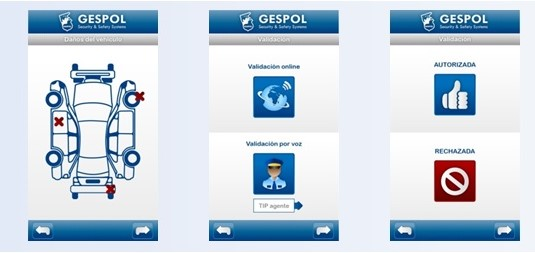
\includegraphics[scale=0.75]{imagenes/gespol2.jpg}
	\caption{Validación de usuario y daños de vehículos en GESPOL.\cite{gespol} \label{fig:figura16}}
\end{figure}

\begin{figure}[H]
	\centering
	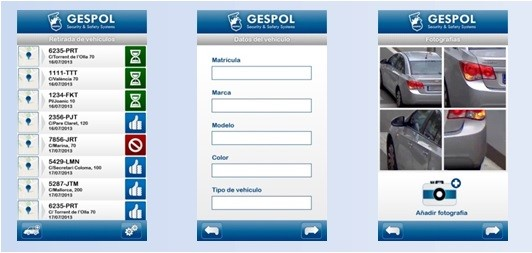
\includegraphics[scale=0.75]{imagenes/gespol1.jpg}
	\caption{Retirada, daños y fotografías de vehículos en GESPOL.\cite{gespol} \label{fig:figura17}}
\end{figure}

El principal problema de esta aplicación es que está bastante desactualizada. El desarrollo se terminó y no se han incluido mejoras en el software. Además,
es una aplicación de pago y no es de código libre, por lo que no la podemos utilizar para continuar su desarrollo con nuevas funcionalidades y adaptada a las tecnologías recientes.

\section{Appolo}
La segunda aplicación a analizar se llama \textbf{Appolo} y ha sido creada por la empresa \textit{Almerimatik Sistemas Informáticos S.A}. \\

\textit{Appolo} es un sistema informático para la gestión completa de los Cuerpos de Policía Local y afirman que es un sistema
flexible, abierto y que están en permanente evolución debido a las necesidades de sus usuarios.\\

Algunas de las funcionalidades que ofrece son las siguientes:
\begin{itemize}
	\item Gestiona el seguimiento de la actividad de los agentes.
	\item Permite completar todo el ciclo de las sanciones de ordenanza, de tráfico y de O.R.A. 
	\item Posee un módulo de sala para organizar el trabajo de los agentes.
	\item Los agentes pueden generar denuncias y partes.
	\item Es multi-entidad, por lo que se puede usar en distintas jefaturas.
\end{itemize}

En la siguiente imagen se puede comprobar los bloques en los que se compone:

\begin{figure}[H]
	\centering
	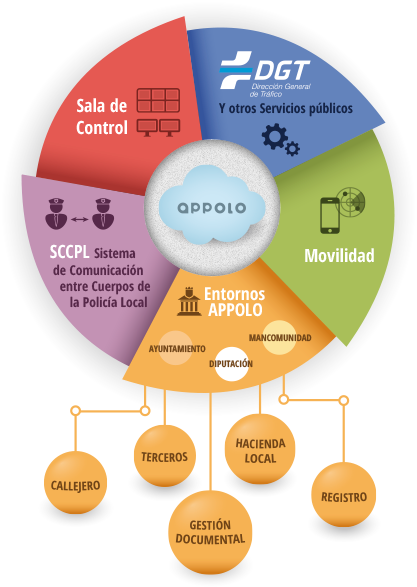
\includegraphics[scale=0.55]{imagenes/appolo-info.png}
	\caption{Bloques que conforman Appolo.\cite{appolo} \label{fig:figura15}}
\end{figure}

Esta aplicación se rige bajo una licencia \textit{open source} pero bajo pago. Por tanto, no podemos conocer el código de la aplicación
sin haber pagado por la licencia. El sistema de cobro que usan es el basado en tarifa plana, por lo cual se deberá pagar en un
único plazo y antes de comenzar a utilizar la aplicación. Esto ocasiona una gran barrera en el momento de querer comenzar a utilizar esta aplicación ya que hasta que no obtenemos la licencia, no podremos saber si se adapta a las necesidades que tenemos o si es realmente útil para los agentes.

\section{Crítica al estado del arte}

Después de analizar las aplicaciones anteriores, se puede concluir que \textbf{no} existe una aplicación
de código libre, gratuita y en la que los desarrolladores de la comunidad puedan involucrarse de manera activa.
Las aplicaciones anteriores no son muy usadas debido a su alto precio. En la mayoría de los casos, las instituciones
no pueden permitirse este gasto y no cambian el modelo que están utilizando actualmente.\\


Con esta aplicación se podrá llegar donde las anteriores aplicaciones no han llegado. De este modo al tener en cuenta un mayor sector de posibles usuarios, 
\textbf{Chief} puede conseguir una mayor implantación en el mercado. Esto puede provocar que la comunidad de desarrolladores vea una buena oportunidad y se involucre 
de manera activa en el proyecto, consiguiendo mejoras y atendiendo a las necesidades de la comunidad.

\section{Propuesta}

Se propone crear el \textbf{primer} sistema de ayuda a la labor policial de código libre y completamente gratuito que cuente
con el apoyo directo de una institución del Estado. Este proyecto puede significar una gran paso para la aceptación 
del código libre como una alternativa igual de válida que el código cerrado para un sector en el 
que hasta ahora, no ha tenido cabida.\\  

	
	\chapter{Planificación}
\section{Metodología utilizada}

Para el desarrollo de este trabajo se ha utilizado una metodología ágil y, en concreto, se ha optado por una versión personal basada en \textit{Scrum}\cite{scrum}. En esta metodología
ágil propia, se sigue un desarrollo por pequeñas funcionalidades que se deben resolver en pequeños periodos de tiempo llamados \textit{sprints}. Para organizar los contenidos, así como las tareas
a realizar y el progreso de cada una, se ha utilizado la funcionalidad de \textbf{Proyectos} de GitHub, en la cual las tareas se han dividido en 3 secciones. Estas tareas
quedan representadas por \textit{issues}, que se utilizan para llevar un progreso del desarrollo. La lista completa de \textit{issues} se puede encontrar \href{https://github.com/Cerv1/Chief/issues?q=is\%3Aissue+is\%3Aclosed}{aquí.} \\

Estos \textit{issues} estarán dentro del proyecto en uno de los 3 estados siguientes:

\begin{itemize}
	\item \textbf{Por hacer.} Aún no se ha comenzado el desarrollo de la nueva funcionalidad, el arreglo de un fallo o la actividad a la que referencie el \textit{issue}.
	\item \textbf{En progreso.} Actualmente se está trabajando para terminar el objetivo por el cual ha sido abierto el \textit{issue}.
	\item \textbf{Finalizado. } El desarrollo correspondiente a la actividad ha sido terminado y se ha incorporado al código fuente de la aplicación.
\end{itemize}

Además, estos \textit{issues} se han agrupado dentro de \textit{milestones} o hitos, los cuales serán definidos en capítulos posteriores.\\

Este tipo de metodología ayuda a conseguir un progreso coherente y más acertado. Esto se debe a que es más fácil estimar la cantidad de tiempo que se requerirá para
implementar una pequeña funcionalidad o solucionar un error que incluir un sistema completo y muy complejo. Otra ventaja de seguir esta metodología es que se puede ver
un desarrollo realista de la aplicación desde el principio hasta el final. Se puede comprobar en qué punto se incluyó exactamente qué funcionalidad y cuanto tiempo de 
trabajo requirió. 

\section{Temporización}
La planificación temporal que se ha establecido durante el desarrollo ha sido la siguiente:

\renewcommand{\arraystretch}{1.5}
\begin{table}[H]
	\centering
	\label{tabla-temporal}
	\resizebox{\textwidth}{!}{%
	\begin{tabular}{@{}ccc@{}}
		\toprule
		\rowcolor[HTML]{ECF4FF} 
		\textbf{Etapas del desarrollo}                                                                                                                  & \textbf{Fecha de comienzo} & \textbf{Fecha de finalización} \\ \midrule
		\cellcolor[HTML]{ECF4FF}\textbf{\begin{tabular}[c]{@{}c@{}}Reuniones iniciales para realizar\\ las especificaciones del proyecto.\end{tabular}} & 19 de Marzo                & 2 de Abril                     \\
		\rowcolor[HTML]{EFEFEF} 
		\cellcolor[HTML]{ECF4FF}\textbf{Planificación de los contenidos}                                                                                & 3 de Abril                 & 10 de Abril                    \\
		\cellcolor[HTML]{ECF4FF}\textbf{\begin{tabular}[c]{@{}c@{}}Análisis y diseño tanto del problema\\ como de las soluciones.\end{tabular}}         & 11 de Abril                & 22 de Abril                    \\
		\rowcolor[HTML]{EFEFEF} 
		\cellcolor[HTML]{ECF4FF}\textbf{Implementación del software.}                                                                                   & 22 de Abril                & 1 de Junio                     \\
		\cellcolor[HTML]{ECF4FF}\textbf{Pruebas en un entorno controlado.}                                                                              & 1 de Junio                 & 7 de Junio                     \\
		\rowcolor[HTML]{EFEFEF} 
		\cellcolor[HTML]{ECF4FF}\textbf{Documentación.}                                                                                                 & 2 de Junio                 & 15 de Junio                    \\ \bottomrule
	\end{tabular}}
	\caption{Tabla con la organización temporal del proyecto.}
\end{table}

Como se puede comprobar, el proceso de elaborar esta documentación comenzó al mismo tiempo que las pruebas en un entorno controlado. Esto se debe a que a partir de este punto, 
no se iba a incorporar más funcionalidad al software y por tanto, se podía comenzar a planear la documentación, preparar las plantillas de LaTeX y organizar el contenido.

\section{Seguimiento del desarrollo}
Para llevar un correcto seguimiento del desarrollo, se ha planificado una reunión todos los Lunes con el tutor de dicho trabajo, D. Juan Julián Merelo. En estas pequeñas 
tutorías se presentaban las mejores y se comentaba el trabajo a desarrollar durante la siguiente semana. Además, su opinión ha sido de gran utilidad a la hora de descubrir
nuevas herramientas o utilizar las ya existentes de una mejor manera.\\

Gracias a estas reuniones se ha podido llevar un seguimiento del proceso de creación, desde el comienzo hasta el final de su etapa.


	% Análisis del problema
	% 1. Análisis de requisitos
	% 2. Análisis de las soluciones
	% 3. Solucion propuesta
	% 4. Análisis de seguridad
	\chapter{Análisis del problema}
 
 Como todo software, esta aplicación se ha diseñado y desarrollado para cubrir unas necesidades muy bien definidas. En base a dicha premisa, podemos crear una descripción completa de los 
 actores, así como una lista de requisitos detallada con la que se cubran los objetivos previamente
 propuestos.

\section{Descripción de los actores}
Vamos a disponer de dos actores: el \textbf{usuario} y el \textbf{administrador}.\\

El \textbf{usuario} será el agente de policía que desee realizar cualquiera de las acciones
disponibles en la aplicación. Este actor no tiene por qué tener ninguna experiencia previa
con aplicaciones web, pero en este escenario se les ha formado con unas nociones básicas 
a modo de tutorial de cómo realizar todas las acciones posibles en la aplicación y las consecuencias
que tiene en el servidor. De esta manera, el usuario no tiene ningún problema interaccionando con la aplicación.\\

El \textbf{administrador} será la persona encargada de asegurar el correcto funcionamiento 
del software así como el encargado de la gestión de los datos de usuario y de la aplicación. Este
actor, por tanto, debe tener un alto conocimiento de las tecnologías con las que se ha construido
\textbf{Chief} para poder dar una rápida respuesta a los posibles problemas del usuario.

\section{Análisis de requisitos}

Los requisitos serán divididos en 3 tipos:

\begin{itemize}
   \item \textbf{Requisitos funcionales:} Son servicios que el sistema debe proporcionar, cómo
   debería responder a entradas concretas y como debe reaccionar el sistema en situaciones 
   particulares. En algunos casos, se puede especificar explícitamente qué no debe hacer el sistema.\cite{software-engineering}

   \item \textbf{Requisitos no funcionales:} Son requisitos que no tienen que estar directamente relacionado
   con el funcionamiento de la aplicación, sino más bien con el proceso del desarrollo.
   
   \item \textbf{Requisitos de información:} Estos requisitos están relacionados con la información 
   que se va a guardar en el sistema.
\end{itemize}

Para el siguiente punto se utilizarán las siguientes abreviaturas:\\
\renewcommand{\arraystretch}{1.5}
\begin{table}[H]
   \centering
   \label{tabla-abreviaturas}
   \begin{tabular}{|c|l|}
   \hline
   \textbf{Abreviatura} & \textbf{Significado} \\ \hline
   R.F X       & Para denotar el requisito funcional número \textit{X}.\\ \hline
   R.F X.Y     & Para denotar el subrequisito funcional número \textit{Y} de \textit{X}\\ \hline
   R.F X.Y.Z   & Para denotar el subrequisito funcional número \textit{Z} de \textit{Y}\\ \hline
   R.N.F X     & Para denotar el requisito no funcional número \textit{X}\\ \hline
   R.N.F X.Y   & Para denotar el subrequisito no funcional número \textit{Y} de \textit{X}\\ \hline
   R.N.F X.Y.Z & Para denotar el subrequisito no funcional número \textit{Z} de \textit{Y}\\ \hline
   R.I X       & Para denotar el requisito de información número \textit{X}\\ \hline
   R.I X.Y     & Para denotar el subrequisito de información número \textit{Y} de \textit{X}\\ \hline
   R.I X.Y.Z   & Para denotar el subrequisito de información número \textit{Z} de \textit{Y}\\ \hline
   \end{tabular}
   \caption{Tabla de abreviaturas para los tipos de requisitos.}
\end{table}


\subsection{Requisitos funcionales}
Los requisitos funcionales del desarrollo son los siguientes: 

\begin{itemize}
	
	\item \textbf{R.F 1}. Administración de los agentes.
	\begin{itemize}
		\item \textbf{R.F 1.1}. Registro de los agentes.
		\item \textbf{R.F 1.2}. Acceso de los agentes.
		\item \textbf{R.F 1.2}. Cerrar sesión.
	\end{itemize}

	\item \textbf{R.F 2}. Administración de turnos.
	\begin{itemize}
		\item \textbf{R.F 2.1}. Crear un documento de turno.
		\item \textbf{R.F 2.2}. Crear una nueva incidencia.
		\item \textbf{R.F 2.3}. Finalizar un parte de servicio.
	\end{itemize}

	\item \textbf{R.F 3}. Creación de ordenanzas.
	\begin{itemize}
		\item \textbf{R.F 3.1}. Crear una ordenanza de limpieza.
		\item \textbf{R.F 3.2}. Crear una ordenanza de ruidos.
		\begin{itemize}
			\item \textbf{R.F 3.2.1}. Crear un acta de molestias de ruidos en la vía pública.
			\item \textbf{R.F 3.2.2}. Crear un acta de molestias de ruidos en domicilio.
			\item \textbf{R.F 3.2.3}. Crear un acta de molestias de ruidos en local.
			\item \textbf{R.F 3.2.4}. Crear un acta de medición de ruidos.
		\end{itemize}
		\item \textbf{R.F 3.3}. Crear una ordenanza de obras.
		\begin{itemize}
			\item \textbf{R.F 3.3.1}. Crear un acta inspección de obras.
		\end{itemize}
		\item \textbf{R.F 3.4}. Crear una ordenanza de residuos.
		\begin{itemize}
			\item \textbf{R.F 3.3.1}. Crear un acta hallazgo de residuos.
		\end{itemize}
	\end{itemize}

	\item \textbf{R.F 4}. Creación de partes de accidentes.
	\begin{itemize}
		\item \textbf{R.F 4.1}. Crear parte de accidente de 2 vehículos.
		\item \textbf{R.F 4.2}. Crear parte de accidente de 3 vehículos.
	\end{itemize}

	\item \textbf{R.F 5}. Administrar croquis.
	\begin{itemize}
		\item \textbf{R.F 5.1}. Crear un croquis.
		\item \textbf{R.F 5.2}. Enviar un croquis.
	\end{itemize}


\end{itemize}

\subsection{Requisitos no funcionales}
Los requisitos no funcionales del desarrollo son los siguientes: 

\begin{itemize}
	\item \textbf{R.N.F 1}. La aplicación se aprovisionará automáticamente.
	\item \textbf{R.N.F 2}. Se utilizarán solamente módulos NPM como dependencias del sistema. 
	\item \textbf{R.N.F 3}. Se desplegará en una máquina virtual en un entorno controlado.
	\item \textbf{R.N.F 5}. Se creará la estructura de directorios necesaria de manera automática. 
	\item \textbf{R.N.F 5}. Para utilizar el sistema de documentos se deberán proporcionar las plantillas.
	\item \textbf{R.N.F 6}. La creación de las máquinas virtuales se realizará automáticamente.
	\item \textbf{R.N.F 7}. La base de datos se creará sin necesidad de administrarla.
\end{itemize}

\subsection{Requisitos de información}
La base de datos de la aplicación almacenará los mínimos datos necesarios, De este modo conseguimos aumentar la seguridad global del sistema:

\begin{itemize}
	\item \textbf{R.I 1}. Datos de usuario.
	\begin{itemize}
		\item Información necesaria para poder identificar a los usuarios del sistema.
		\item ID interno, usuario, contraseña, email, nombre y apellidos.
	\end{itemize}

	\item \textbf{R.I 2}. Datos de incidencias.
	\begin{itemize}
		\item Información necesaria para poder definir correctamente una incidencia dentro de un parte de servicio.
		\item Número identificador, fecha, hora, dependencia, central, número de agente, hecho y actuación.
	\end{itemize}
\end{itemize}

\section{Análisis de las soluciones}

Como en el desarrollo de cualquier software, no existe una solución única. Por tanto, se deben analizar las
distintas tecnologías que hay en el mercado para garantizar que la solución propuesta es la más adecuada para
los problemas que se plantean.

\subsection{Back-end}

\subsubsection{Elección del servidor} 
A la hora de crear una aplicación web, tenemos un amplio abanicos de posibilidades sobre las que crear nuestro servidor. Aunque, en este caso
en concreto, se le ha añadido una restricción y es que el servidor debe ser \textit{open source}. Para obtener
una idea global se puede observar el siguiente gráfico comparativo del uso de distintas tecnologías en los servidores web actuales:

\begin{figure}[H]
	\centering
	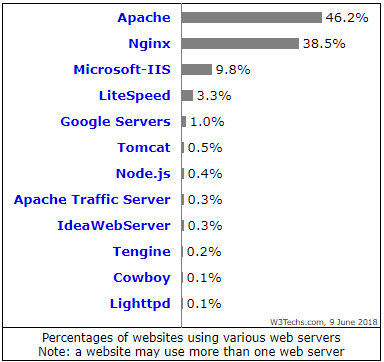
\includegraphics[scale=0.8]{imagenes/web-servers-comparison.png}
	\caption{Comparativa de servidores web.\cite{web-server-usage} \label{fig:figura2}}
\end{figure}

Es inmediato captar la superioridad de Apache\cite{apache} en esta gráfica. Esto se debe, principalmente, a que su lanzamiento 
oficial fue en el año 1996. En esta época no tuvo ningún rival y por tanto se posicionó el primero en el mercado, 
persistiendo aún hoy en día en un gran número de equipos.\\

Sin embargo, en esta lista de servidores todos siguen el esquema tradicional en el que cada petición es atendida 
por una hebra del sistema. En la situación actual del desarrollo web, se está optando por una nueva metodología. La programación
asíncrona orientada a eventos. En este tipo de arquitecturas se consigue un mejor rendimiento con un menor coste 
de recursos debido a la escalabilidad que poseen. \\

En la siguiente imagen podemos ver la diferencia entre un sistema convencional y el utilizado por Node.js\cite{nodejs}.

\begin{figure}[H]
	\centering
	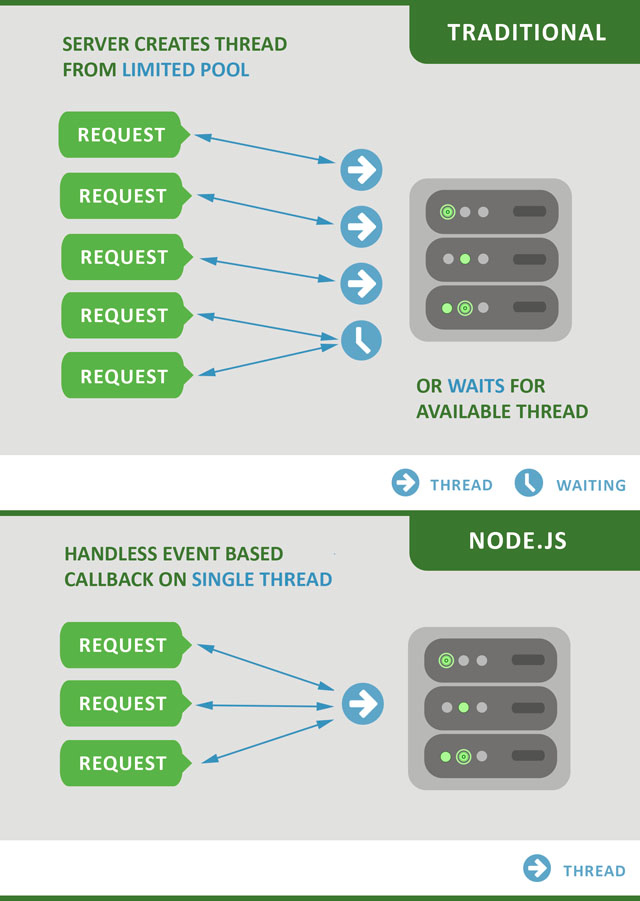
\includegraphics[scale=0.5]{imagenes/traditional-vs-nodejs.jpg}
	\caption{Sistema convencional vs Node \label{fig:figura3}}
\end{figure}

El único servidor web que presenta este tipo de arquitectura es Node.js y es por ello por lo que está
ganando una gran popularidad a medida que pasa el tiempo. Su porcentaje de uso aún es bajo debido a que es una tecnología 
bastante nueva y que está ganando atención en los últimos años, como podemos comprobar en el siguiente gráfico
de tendencia:

\begin{figure}[H]
	\centering
	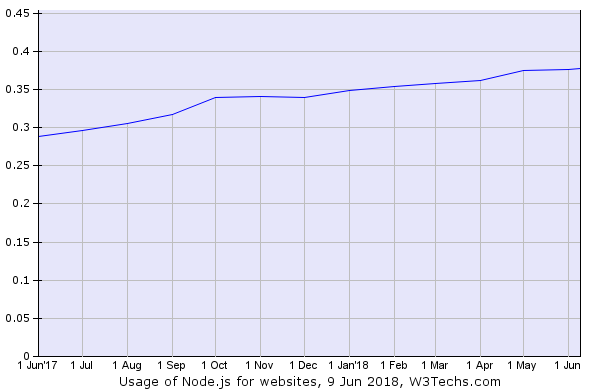
\includegraphics[scale=0.65]{imagenes/nodejs-trend.png}
	\caption{Gráfico de tendencia de Node.js \cite{nodejs-trend} \label{fig:figura4}}
\end{figure}

Además, Node.js dispone de \textit{npm}\cite{npm}, que es la herramienta de gestión de paquetes por defecto de Node. Este
gestor de paquetes fue creado con la intención de ayudar a los desarrolladores de JavaScript  de todo el mundo a compartir y utilizar
módulos de código creados por la comunidad. Lo más destacable de
de este proyecto es la acogida que ha tenido, adquiriendo decenas de miles de usuarios que, además, se involucran
activamente en el desarrollo. De esta manera consiguen una mejora constante del software. Por tanto, se ha logrado conseguir
un gran número de paquetes y hace que el desarrollo con Node sea más liviano, rápido y eficiente. Podemos utilizar paquetes que 
ha desarrollado la comunidad de una manera muy sencilla, ahorrando costes en el tiempo del desarrollo.


\subsubsection{Elección de la base de datos}

En este apartado tenemos dos grandes corrientes: bases de datos relacionales o no relacionales. Dicho de otra manera,
bases de datos \textbf{SQL} o \textbf{NoSQL}. Ambas son opciones completamente válidas pero tienen sus diferencias y serán analizadas a continuación.\\

Las bases de datos SQL utilizan un lenguaje de consulta estructurada (\textit{\textbf{S}tructured \textbf{Q}uery \textbf{L}anguage}) para manipular
y definir los datos. Este tipo de consulta es una de las más usadas y es muy útil para realizar consultas complejas. 
Pero, por otro lado, es muy restrictiva ya que te exige definir la estructura de los datos que se van a almacenar \textbf{antes} 
de realizar cualquier operación y comenzar a trabajar. Esto impacta de manera directa con el tiempo que se debe dedicar a 
la preparación y al planteamiento de los datos que vamos a utilizar y guardar, ya que modificar dicha estructura posteriormente
puede ser realmente costoso y provocar una desestabilización completa de la base de datos.\\

Por otra parte, las bases de datos NoSQL, usualmente llamados \textbf{no sólo SQL}, para destacar que también pueden soportar consultas de tipo SQL. Poseen un esquema dinámico para gestionar los datos no estructurados. Este hecho se puede traducir directamente en las siguientes características:

\begin{itemize}
	\item Se pueden añadir datos sin haber definido previamente su estructura.
	\item Los campos puede cambiar con el tiempo, incluso aparecer o desaparecer.
	\item Cada documento puede tener su propia estructura.
\end{itemize}

Una vez presentadas ambas opciones, podemos comparar sus características y optar por la que mejor se adapte a nuestro producto.

\renewcommand{\arraystretch}{2}
\begin{table}[H]
	\centering
	\resizebox{\textwidth}{!}{%
	\begin{tabular}{@{}ccc@{}}
		\toprule
		\rowcolor[HTML]{ECF4FF} 
		& \textbf{SQL}                                                                                                     & \textbf{NoSQL}                                                                                                               \\
		\cellcolor[HTML]{ECF4FF}\textbf{Datos}        & Estructurados en tablas                                                                                          & Estructuradas en documentos                                                                                         \\
		\rowcolor[HTML]{EFEFEF} 
		\cellcolor[HTML]{ECF4FF}\textbf{Esquema}      & Estático                                                                                                         & Dinámico o flexible                                                                                                          \\
		\cellcolor[HTML]{ECF4FF}\textbf{Escalablidad} & Vertical                                                                                                         & Horizontal                                                                                                                   \\
		\rowcolor[HTML]{EFEFEF} 
		\cellcolor[HTML]{ECF4FF}\textbf{OLTP}         & Recomendada para este tipo de sistemas                                                                           & Menos utilizadas en estos sistemas                                                                                           \\
		\cellcolor[HTML]{ECF4FF}\textbf{Consistencia} & ACID\cite{acid}                                                                                                  & Teorema  CAP\cite{cap}                                                                                                                  \\
		\rowcolor[HTML]{EFEFEF} 
		\cellcolor[HTML]{ECF4FF}\textbf{Rendimiento}  & \begin{tabular}[c]{@{}l@{}}Inversamente proporcional al volumen \\ de datos almacenado actualmente.\end{tabular} & \begin{tabular}[c]{@{}l@{}}Alto y con posibilidad de mejora a costa \\ de reducir la consistencia de los datos.\end{tabular}
	\end{tabular}}
	\caption{Bases de datos SQL vs NoSQL}
\end{table}

Una vez comparadas ambas, podemos comprobar que las bases de datos SQL son especialmente útiles en sistemas robustos, muy bien definidos desde el principio
en el que no se esperan cambios drásticos en la estructura de sus datos. Mientras que las bases de datos NoSQL son útiles cuando buscamos un sistema de se adapte en función de las necesidades del usuario o del propio desarrollo y que además no suponga grandes costes cuando se decida aumentar la escalabilidad del sistema.\\

Por otro lado, también se debe tener en cuenta la \textbf{consistencia} de los datos. Como hemos comprobado, las bases de datos SQL garantizan la consistencia de sus datos por diseño, mientras que en el otro tipo, no se garantiza de un modo tan fiable. Por ello, las bases NoSQL se utilizan cuando manejamos un alto volumen de datos ya que es necesario adaptarse a esta cantidad de tráfico. 


\subsection{Front-end}

Debido a que se a priorizado el desarrollo del \textit{back-end} y su correcto funcionamiento, en esta parte se han optado por tecnologías ya conocidas y utilizadas durante el transcurso del grado.

\subsubsection{Elección del motor de plantillas}

Se ha elegido Pug\cite{pug} ya que es un motor de plantillas de alto rendimiento. Este motor de plantillas era conocido anteriormente como Jade\cite{jade}, pero al tiempo
los desarrolladores se dieron cuenta de que esa marca ya estaba registrada y por tanto tuvieron que cambiar el nombre al proyecto. Cabe destacar,
que debido a la popularidad de Jade, se sigue utilizando en algunas webs pero el paquete ya no cuenta con el soporte oficial y todas las actualizaciones se lanzarán bajo el nuevo nombre. \\

La principal ventaja de este motor de plantillas es su mínima curva de aprendizaje. Esto se debe a que la sintaxis que utiliza es extremadamente sencilla y puede permitir a cualquier usuario crear páginas web en HTML de una manera muy intuitiva como podemos comprobar en el siguiente ejemplo:

\begin{figure}[H]
	\centering
	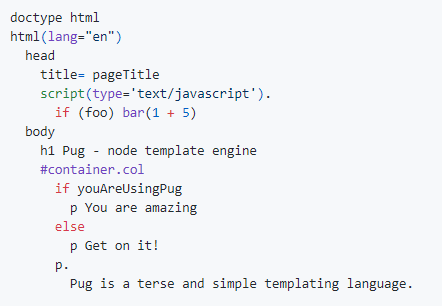
\includegraphics[scale=0.85]{imagenes/pug-example.png}
	\caption{Página de ejemplo escrita en Pug. \label{fig:figura8}}
\end{figure}

Este código será transformado directamente en el siguiente, ya interpretable por el navegador.

\begin{figure}[H]
	\centering
	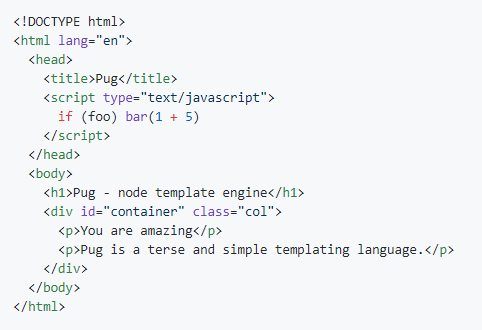
\includegraphics[scale=0.85]{imagenes/pug-rendered.png}
	\caption{Resultado del código ya interpretado. \label{fig:figura9}}
\end{figure}


\subsubsection{Elección del framework CSS}

En \textbf{Chief} se persigue conseguir una interfaz sencilla para que sea lo más simple e intuitiva posible de cara al usuario. De esta manera, la curva de aprendizaje
para utilizar el producto sería mínima. Por tanto, se ha optado por elegir Bootstrap.\\

Boostrap\cite{bootstrap} es la herramienta \textit{open-source} para desarrollo web por excelencia. Es uno de los proyectos libres más populares y utilizado por toda la comunidad.
Fue creado por un trabajador de Twitter a mediados del 2010. Antes de ser el proyecto libre que es ahora, era privado ya que Twitter poseía los derechos sobre el mismo.
Pero todo cambió cuando Twitter celebró su primera Hack Week\cite{hack-week} y vieron la acogida del proyecto por parte de toda la comunidad de desarrolladores. Siguió en desarrollo
durante un año después de dicho evento y, finalmente, se publicó la primera versión del \textit{framework} tan conocido a día de hoy.\\

Debido a su simpleza a la hora de ser utilizado y a lo sencilla que es su sintaxis, se pueden crear páginas web completamente adaptables de una manera muy rápida e intuitiva. Además, al ser tan conocido en la comunidad hay una gran cantidad de tutoriales en los que se enseña a utilizarlo desde 0.

\newpage

\section{Solución propuesta}

En base al análisis anterior, se ha decidido utilizar como dato base para la aplicación JSON\cite{json}.\\

El motivo principal es que debido a las características del desarrollo a realizar y los requerimientos del sistema,
una base de datos \textbf{NoSQL} era la opción idónea para este software. Esto es debido a que como hemos comprobado,
es una base de datos muy flexible, que permite la incorporación de nuevos campos sin provocar grandes problemas en 
la base de datos ni desestructurarla por completo.\\

Además, dado que el objetivo del desarrollo es conseguir un prototipo funcional, con el tiempo se le podrán añadir
nuevas funcionalidades, nuevos tipos de usuarios, nuevos campos a las incidencias... Por tanto, para garantizar 
la consistencia del sistema en un futuro se ha optado por este tipo de base de datos.\\

Finalmente, después de un estudio completo de las tecnologías más usadas actualmente en aplicaciones con unas características similares a \textbf{Chief}, la solución al problema inicial se ha conseguido 
mediante el uso de las siguientes tecnologías.

\subsection{Node.js}

Node.js es un entorno de ejecución para JavaScript construido con el motor de JavaScript
V8 de Chrome. En este proyecto se ha utilizado para elaborar el servidor de la aplicación.\\

Node.js tiene una característica que lo diferencia del resto de posibilidades para implementar 
el servidor, como comentamos anteriormente, y es que utiliza un modelo de operaciones E/S sin bloqueo y orientado a eventos 
\textbf{asícronos}. Esto nos ofrece la posibilidad de que cuando se detecte una conexión se atienda
pero el resto del tiempo estará inactivo, no malgastando potencia de computo ni energía. Con este nuevo modelo conseguimos servidores altamente 
escalables de una manera muy sencilla, rápida y eficiente.\\

\begin{figure}[H]
	\centering
	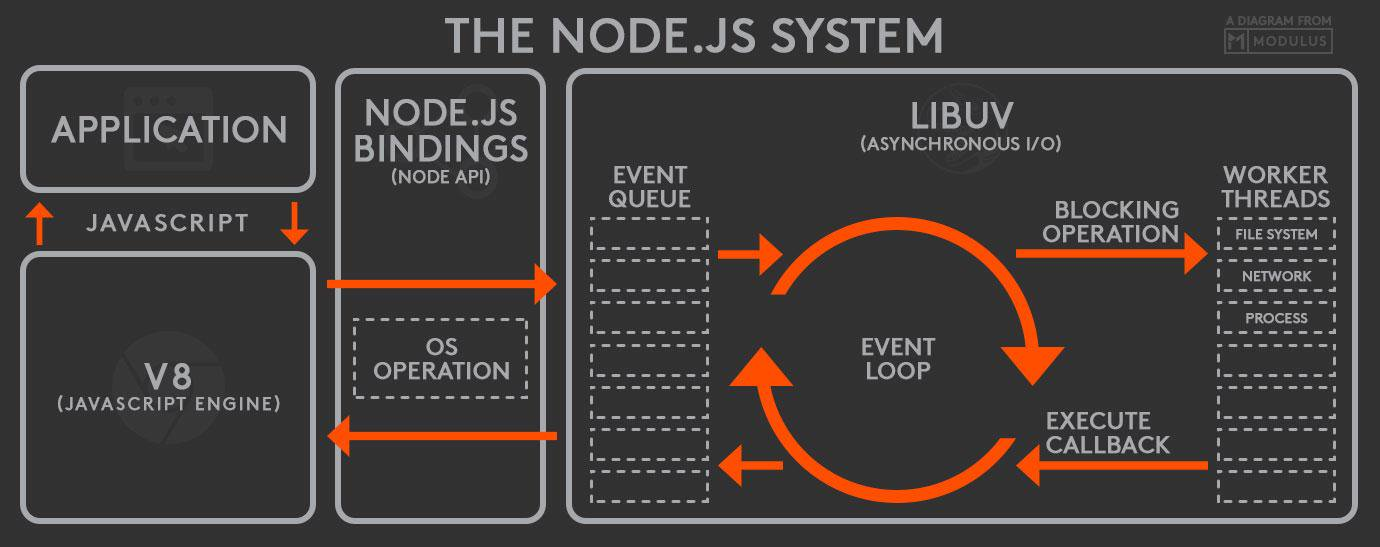
\includegraphics[scale=0.25]{imagenes/nodejs_system.jpg}
	\caption{Sistema de Nodejs \label{fig:figura1}}
\end{figure}

Este diseño contrasta directamente con el modelo de concurrencia más común hoy en 
día en el que se usan hilos del Sistema Operativo para resolver peticiones. Las operaciones en red basadas en este modelo son relativamente ineficientes además de complejas en su uso. Cabe mencionar que, aunque Node.js 
no utilice hilos del Sistema Operativo del mismo modo que los servidores clásicos, no implica que no podamos aprovechar los múltiples núcleos de nuestro sistema.\\

Otro punto a favor de Node.js es que no tendremos que preocuparnos por la posibilidad de un 
bloqueo en el proceso debido a que no existe dicha posibilidad por la naturaleza de dicha 
tecnología, la cual, como se ha comprobado, está basada en un bucle de eventos.

\subsection{MongoDB}

MongoDB es un sistema de base de datos multiplataforma y orientado a documentos de esquema libre.
Esto quiere decir que cada entrada puede tener un esquema de datos diferente al anterior, por
lo que podemos tener entradas que difieran en el número de atributos entre sí.\\

Debido a esta característica los datos no son guardados en registros, como en las bases SQL, 
sino que se guardan en documentos. Estos archivos son del tipo BSON, que es una representación
binaria de los archivos JSON.\\

Esta tecnología ha sido escrita en C++, por lo que está en contacto con el \textit{bare metal}. Esto
último es realmente importante ya que le permite optimizar los recursos y acceder a ellos de una 
manera extremadamente eficiente, con lo que consigue una velocidad muy alta en todas sus operaciones.\\

Cabe mencionar que MongoDB es una plataforma completamente distribuida, lo que nos proporciona 
un nuevo nivel de escalabilidad y disponibilidad. Esto quiere decir que a medida que nuestro desarrollo
crezca tanto en volumen de datos como en rendimiento MongoDB se escala automáticamente sin tiempos
de caída y sin cambios en nuestra aplicación.\\

Mediante la utilización del paquete de \textit{npm} llamado \textit{Mongoose}\cite{mongoose}, la integración de MongoDB
con Node.js se realiza de una manera muy sencilla y rápida, por lo que la utilización de este módulo
cuando trabajamos con ambas tecnologías es ideal. En la siguiente imagen se define el flujo de datos
estándar cuando trabajamos con este esquema:

\begin{figure}[H]
	\centering
	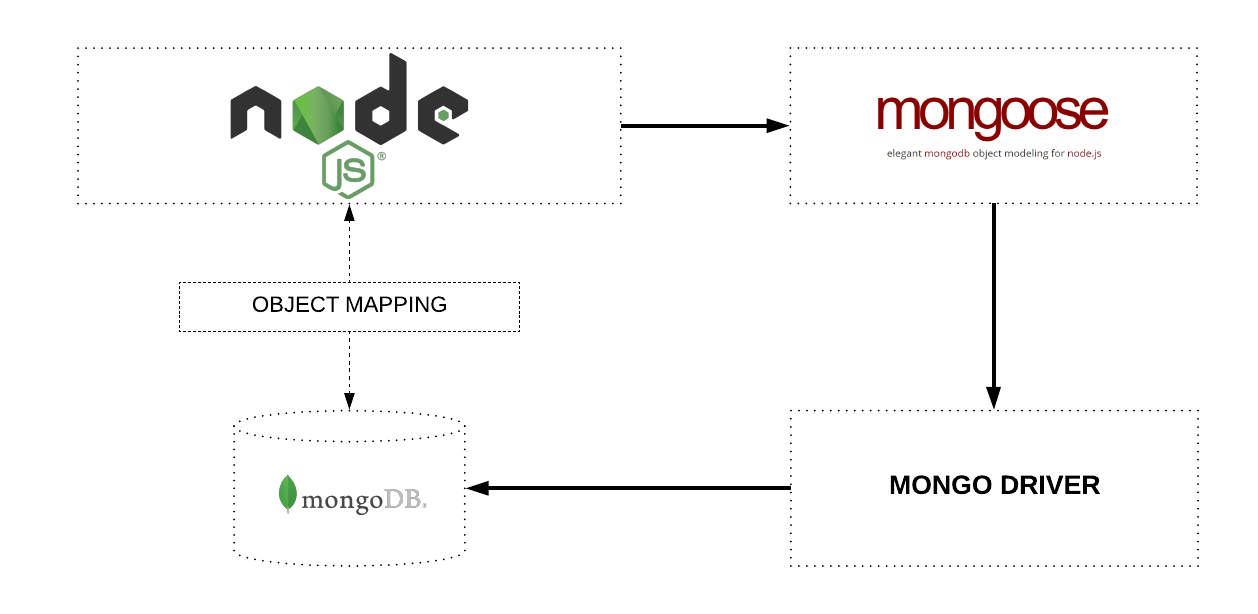
\includegraphics[scale=0.28]{imagenes/node-mongo.png}
	\caption{Flujo de datos con Node.js, Mongoose y MongoDB. \label{fig:figura5}}
\end{figure}


Por último, cabe mencionar que la licencia de esta tecnología es GNU AGPL 3.0\cite{agpl}, por lo que se trata de un software con licencia
libre.


% gráficas de uso frente al resto de bbdd

\subsection{Vagrant}

Vagrant\cite{vagrant} es una herramienta creada para construir y administrar entornos de máquinas virtuales de una 
manera sencilla. Debido a que está diseñado para ser sencillo de utilizar y a que se centra en 
la automatización hace que utilicemos el menor tiempo posible en la preparación del entorno virtual
que necesitamos para comenzar a trabajar.\\

Nos proporciona un entorno muy rápido y simple de configurar, reproducible y portable utilizando
tecnología puntera en el sector de la virtualización como puede ser VirtualBox, VMWare, AWS, Docker...\\

Una enorme ventaja que aporta Vagrant al desarrollo es la posibilidad de aislar toda la configuración
del entorno y todas sus dependencias. Además, no hay que cambiarlas herramientas de trabajo usuales, pues realmente se sigue trabajando en la misma máquina. 
De esta manera se consigue un desarrollo más eficiente y con mínimas pérdidas de tiempo, garantizando 
de manera directa una eficiencia en la gestión de los recursos humanos empleados.\\

En la siguiente imagen se puede ver como funciona el flujo de trabajo utilizando esta herramienta:

\begin{figure}[H]
	\centering
	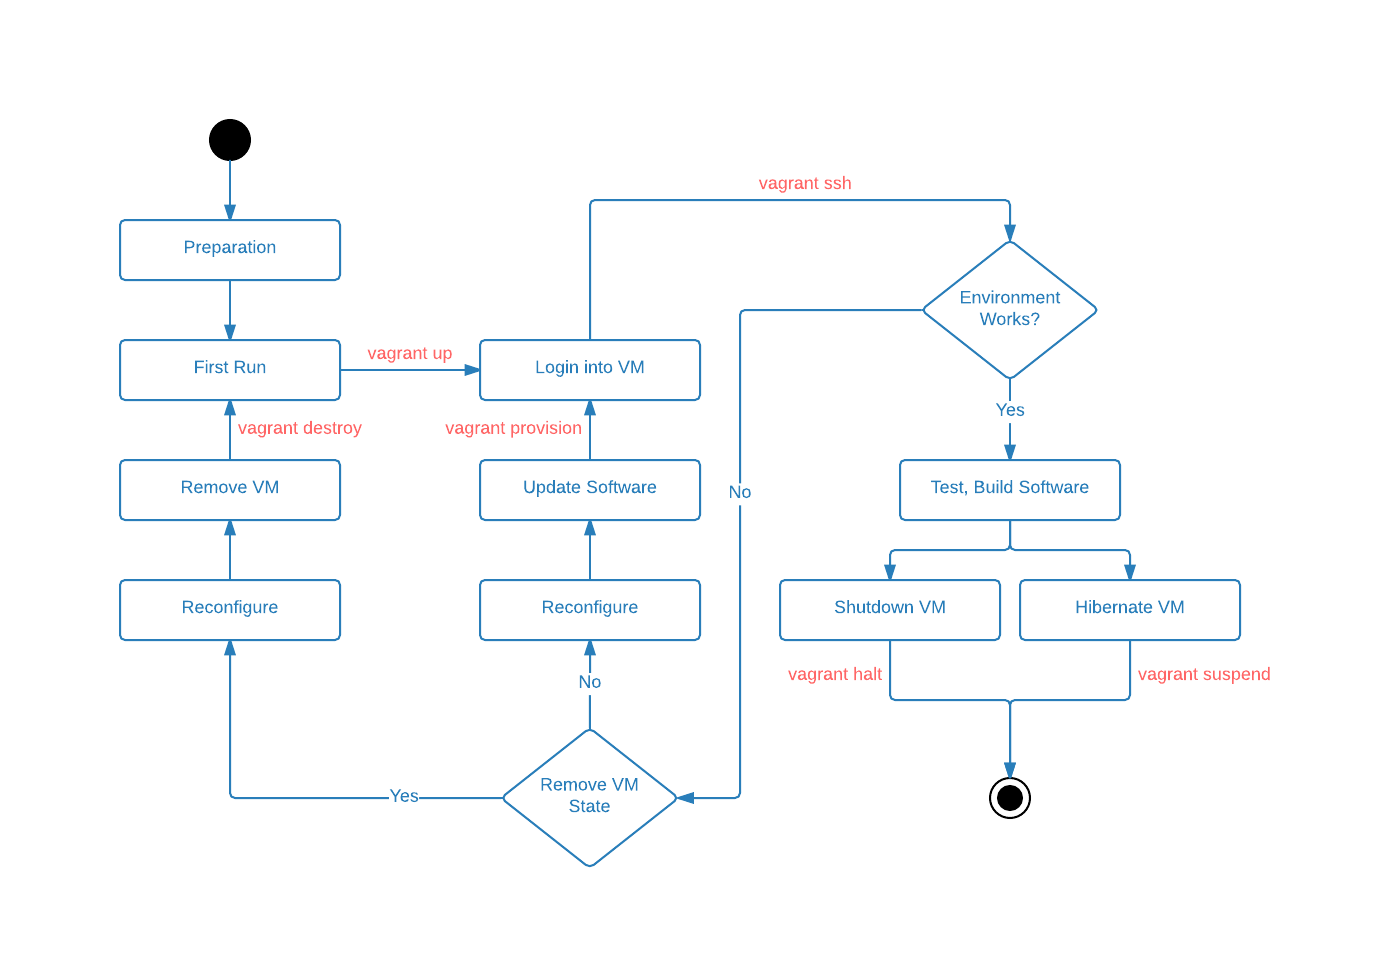
\includegraphics[scale=0.65]{imagenes/vagrant-workflow.png}
	\caption{Flujo de trabajo de Vagrant. \label{fig:figura6}}
\end{figure}


\subsection{Ansible}

Ansible\cite{ansible} es un software que se ha diseñado explícitamente para automatizar acciones y
conseguir una mayor productividad. De esta manera, se libera al equipo de tareas costosas
y que siempre siguen el mismo proceso.\\

Ansible está categorizado bajo el nombre de \textbf{herramienta de orquestación} debido a 
las funciones que realiza. Se encarga de manejar nodos a través de \textit{SSH} habiendo recibido
una entrada por parte del usuario. De esta manera, se le proporciona una entrada muy sencilla
y comprensible para la lectura del ser humano, que posteriormente es analizada y transformada
en una serie de tareas hacia los nodos, consiguiendo quedar completamente configurados de una
manera eficiente.\\

\begin{figure}[H]
	\centering
	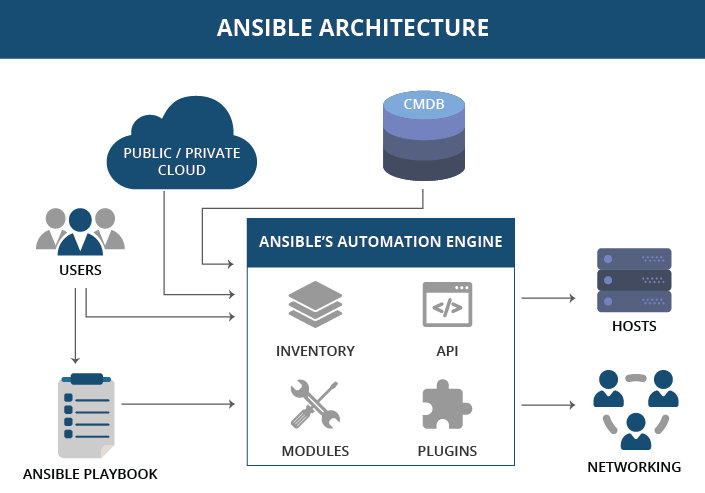
\includegraphics[scale=0.45]{imagenes/ansible.png}
	\caption{Arquitectura de Ansible. \label{fig:figura7}}
\end{figure}

Como podemos comprobar en la figura anterior, Ansible se encarga de realizar todas las acciones
necesarias para que nuestro software esté listo para desplegarse \textbf{de manera automática}.
De este modo, se conseguirá una mejora significable en el tiempo de despliegue de una aplicación
además de en la gestión del tiempo de los desarrolladores.\\

Es la herramienta de automatización de código libre más potente actualmente y esto es reflejado
en las estadísticas de GitHub del proyecto. Además, la comunidad está implicada muy directamente
en el desarrollo de esta herramienta ya que cuenta con más de 2.400 personas que han desarrollado
uno o varios módulos para mejorarla.

\subsection{Carbone}
Carbone\cite{carbone} no es una herramienta más en el desarrollo de la aplicación. Su uso deriva de la inexistencia de un sistema de gestión documental libre que ofrezca la posibilidad de administrar, rellenar y almacenar las plantillas necesarias. Por tanto, utilizando \textit{Carbone} como base se ha realizado un sistema de gestión documental a medida para este proyecto, consiguiendo todas las funcionalidades nesearias para el correcto funcionamiento de la aplicación y de una manera libre y gratuita.\\

Carbone es una herramienta que permite la inyección de datos en documentos provenientes tanto de LibreOffice como de Microsoft Office, aceptando por tanto la gran mayoría de documentos de texto. De hecho, funciona con todos los documentos basados en el formato \textit{XML}, por lo que su alcance no solo se remite a los programas y formatos previamente mencionados.\\

Esta herramienta es la que ha conseguido que se puedan generar documentos de texto rellenos con los datos adquiridos a través de la aplicación web. Su funcionamiento es simple.\\

\begin{enumerate}
	\item \textbf{Lee una plantilla adaptada.} Le indicamos donde se encuentra la plantilla sobre la que queremos escribir. 
	\item \textbf{Analiza el documento.} Analiza completamente la plantilla en busca de los marcadores \{ y \}.  
	\item \textbf{Recibe los datos en formato \textit{JSON}.} Nuestra aplicación le proporciona los datos que queremos inyectar en el documento con formato \textit{JSON}.  
	\item \textbf{Inyecta los datos.} Realiza una sustitución del contenido de nuestros datos en los marcadores que ha encontrado previamente sobre el documento.
	\item \textbf{Escribe en el fichero destino.} Una vez realiza las sustituciones, procede a escribir el documento resultante en el disco. 
\end{enumerate}

Además de realizar sustituciones, esta herramienta se puede utilizar para dar formato a los datos, repetir porciones del documento como pueden ser filas de una tabla, añadir lógica a la inyección de los datos... Para ayudar a la comprensión, se presenta el siguiente caso de uso real como ejemplo:\\

\textit{Nuestra aplicación genera el siguiente archivo en formato JSON después de que un agente haya rellenado los datos de un formulario.}

\begin{figure}[H]
	\centering
	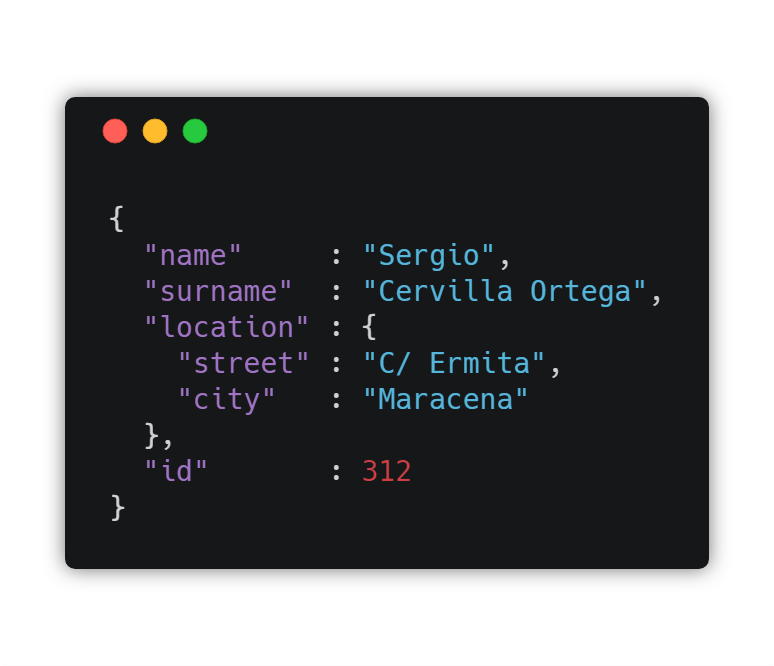
\includegraphics[scale=0.4]{imagenes/json-carbone.png}
	\caption{JSON generado por la aplicación \label{fig:figura10}}
\end{figure}
\newpage

\textit{Una vez disponemos del archivo JSON con los datos, lo utilizamos junto a la plantilla en la que queremos escribir el contenido de dicho archivo, que tendrá el siguiente formato: }

\begin{figure}[H]
	\centering
	\resizebox{\textwidth}{!}{%
	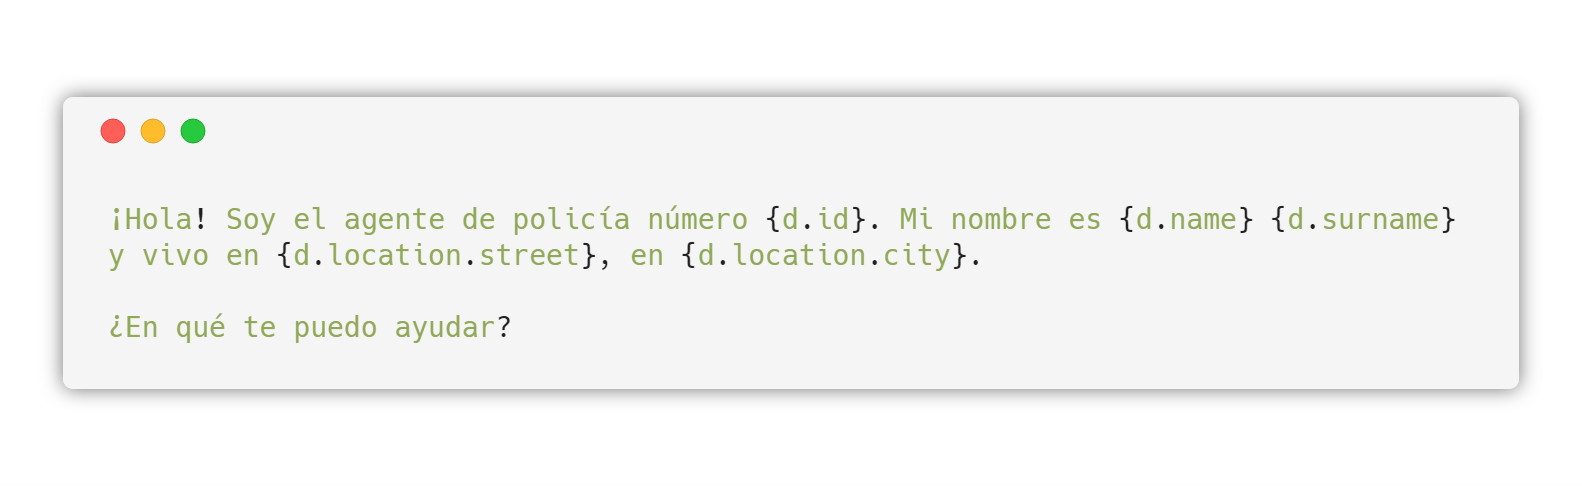
\includegraphics{imagenes/carbone-template.png}}
	\caption{Plantilla sobre la que inyectar los datos. \label{fig:figura11}}
\end{figure}

\textit{Una vez procesados los datos sobre la plantilla, obtendremos el siguiente documento:}
\begin{figure}[H]
	\centering
	\resizebox{\textwidth}{!}{%
		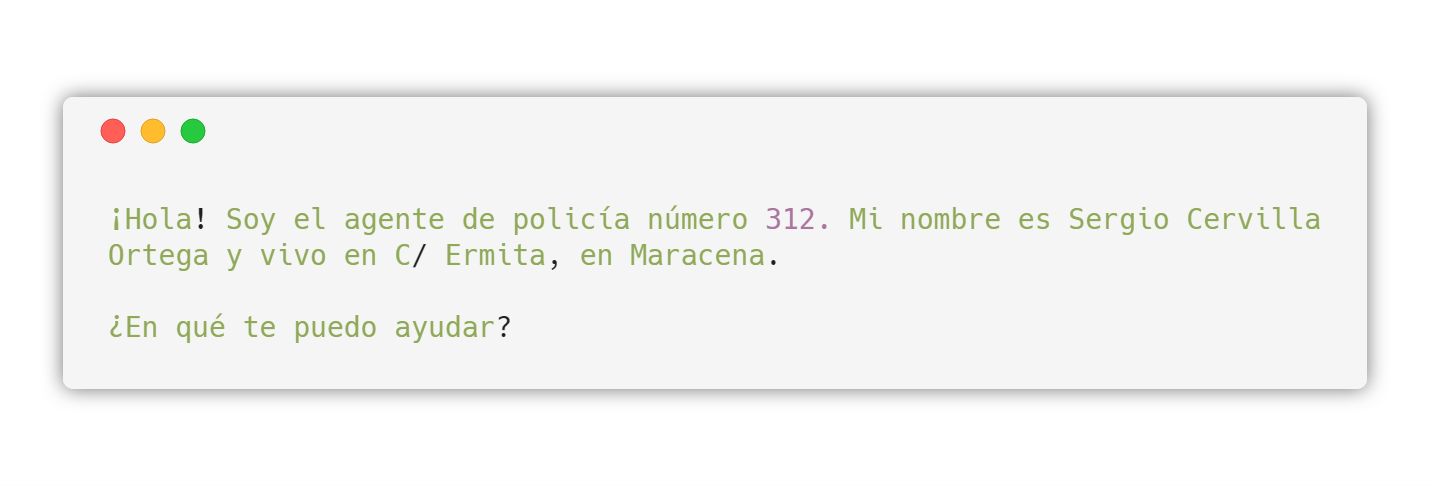
\includegraphics{imagenes/carbone-result.png}}
	\caption{Resultado final tras usar Carbone. \label{fig:figura12}}
\end{figure}

Con este ejemplo, queda claro el uso que tiene en \textbf{Chief} y lo sencillo que es de utilizar esta herramienta para generar documentos de texto rellenos mediante inyección de datos.

	


	% Desarrollo bajo sprints: 
	% 	1. Permitir registros y login de usuarios
	% 	2. Desarrollo del sistema de incidencias
	% 	3. Desarrollo del sistema de denuncias administrativas y accidentes
	% 	4. Desarrollo del sistema de croquis
	%   5. Instalación de la aplicación de manera automática
	\chapter{Implementación}

La implementación del software se ha dividido en hitos. Estos, han sido definidos en Github
y cada uno de ellos contiene un grupo de \textit{issues} que se corresponden con las distintas
mejoras que se han ido incorporando al software a lo largo de su desarrollo.\\

Los hitos han sido los siguientes en orden cronológico:

\begin{enumerate}
	\item \textbf{Permitir registros y acceso de usuarios.}
	\item \textbf{Desarrollo del sistema de documentación.}
	\item \textbf{Desarrollo del sistema de croquis.}
	\item \textbf{Desarrollo del sistema de tests unitarios.}
	\item \textbf{Integración continua.}
	\item \textbf{Instalación de la aplicación de manera automática.}
\end{enumerate}

Toda la información relacionada con la implementación y el desarrollo se pueden encontrar en:

\begin{itemize}
	\item \href{https://github.com/Cerv1/Chief/milestones}{Lista de hitos.}
	\item \href{https://github.com/Cerv1/Chief/commits}{Lista de commits.}
\end{itemize}

\newpage

\section{Registro y acceso de usuarios.}
El objetivo de este hito es permitir que un usuario agente cree una cuenta en la aplicación 
y posteriormente pueda acceder a la misma si la contraseña y el usuario es válido. \\

Para poder utilizar el servidor de una manera más cómoda y con un mayor número de funcionalidades se ha utilizado
\textbf{Express.js}\cite{express} para crear el servicio web que se ofrece. De esta manera, conseguimos utilizar el 
servidor de una manera más eficiente.\\

Express.js ofrece un software liviano que dota de funcionalidades como negociación de contenido, una mejora en el 
rendimiento del servidor, la posibilidad de seleccionar un motor de plantillas para servir el contenido... En este caso,
se ha configurado para que utilice como motor de plantillas el ya mencionado \textbf{Pug}. De esta manera, cuando el usuario
realice una petición sobre alguna ruta se traducirá dicha plantilla para que el usuario reciba el archivo HTML, el cual
será interpretado por el navegador que esté utilizando.\\ 

Un usuario que quiera acceder a la aplicación o a cualquiera de las funcionalidades que ofrece deberá estar \textbf{autenticado}.
Para administrar de una manera más segura los datos de sesión de un usuario se ha utilizado la biblioteca \textbf{Passport.js}\cite{passport}.
Esta biblioteca se encarga de autenticar las peticiones hacia el servidor a través de una serie de \textit{plugins} conocidos
como \textit{strategies}. Gracias al comportamiento de esta biblioteca podemos gestionar de una manera sencilla el acceso a los usuarios.
En este caso, se ha establecido un inicio de sesión mediante \textbf{usuario} y \textbf{contraseña} definidos por el agente en el 
momento de registrarse.\\

En la siguiente imagen se puede comprobar como funciona Passport.js:
\begin{figure}[H]
	\centering
	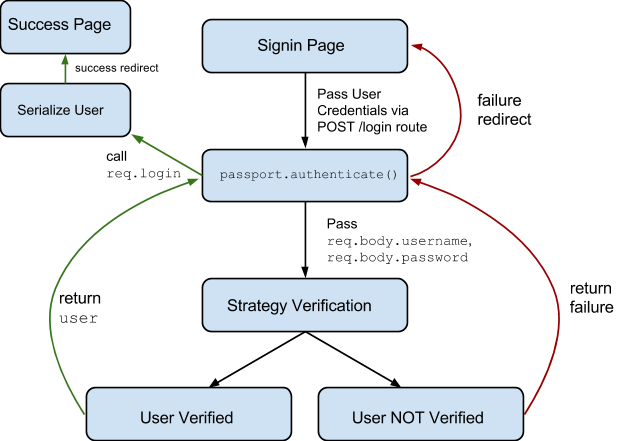
\includegraphics[scale=0.65]{imagenes/passport-auth.png}
	\caption{Esquema del funcionamiento de \textit{Passport.js}\cite{passport-func}. \label{fig:figura18}}
\end{figure}


Cuando un agente realiza un registro, sus datos se almacenan \textbf{encriptados} en la base de datos para que de ninguna manera
se puedan alterar o recuperar de forma fraudulenta. El cifrado de dichos datos se realizan con un algoritmo basado en el cifrado
Blowfish\cite{blowfish} al que se le añaden unos bits aleatorios para proteger nuestro cifrado ante un ataque de Tabla Arcoíris\cite{rainbow}.


\section{Desarrollo del sistema de documentación.}

El primer objetivo de este hito es conseguir un sistema de incidencias completamente funcional y la posibilidad de generar todos los documentos
soportados por la plataforma de manera interactiva y desde cualquier localización. De este modo, se consigue que los agentes aumenten su 
productividad ya que pueden rellenar los documentos de manera inmediata y no tendrán que realizarlo al final del turno.\\

Para la realización de este hito se ha utilizado un módulo completamente propio llamado  \verb|doc_functions.js|. Este módulo ha sido diseñado para ser usado
como biblioteca externa ya que contiene un gran número de funciones para generar los distintos tipos de documentos que podrá manejar la aplicación. De esta manera
se consigue una mejor reutilización del código, además de lograr un menor acoplamiento.\\

Esta biblioteca se encarga de crear el dato de tipo JSON que será posteriormente inyectado en las plantillas. Para ello, tiene en cuenta los datos recibidos
del servidor y otros que gestiona de manera independiente al usuario como pueden ser la fecha, la hora en la que se crea el turno, el formato de salida del 
documento... Además tiene otra función importante y es la de dar feedback al usuario. En la función en la que crea el documento se he creado un \textit{callback}
para poder comunicarse de nuevo con el servidor. De este modo, se podrá saber si la creación del documento ha sido correcta o, por el contrario, si ha fallado.
Podremos utilizar dicho \textit{callback} para devolver un \textit{feedback} al usuario y que sea consciente del resultado de la operación. Por tanto, todas las 
acciones de escritura y creación de documentos han sido desplazadas a dicho módulo, logrando así un mejor diseño y un código mejor estructurado.
\\

Una vez presentado el módulo creado para este hito, se procederá a detallar las funciones que se han creado para el usuario.

\subsection{Comienzo del turno de servicio.}
Cuando el agente desee comenzar un nuevo turno de servicio deberá introducir los datos relacionados con el mismo. Estos datos son los siguientes:

\begin{itemize}
	\item \textbf{Turno.} Podrá ser mañana, tarde o noche.
	\item \textbf{Identificadores de los policías.} Puede ser desde 1 hasta 4 los policías que estén en un turno simultáneamente.
	\item \textbf{Jefe de guardia.} El nombre del agente que actúa como supervisor del turno.
\end{itemize}

Una vez se rellenan estos campos, se creará un nuevo fichero de turno y se rellenarán las cabeceras con los datos anteriormente solicitados.

\subsection{Crear incidencias.}

En este caso, el agente podrá crear un nuevo registro perteneciente a una incidencia que será guardado en la base de datos. Para crear una nueva
incidencia se deberán rellenar los siguientes campos:

\begin{itemize}
	\item \textbf{Número de incidencia.} Número para identificarla. El agente decide que código le asigna.
	\item \textbf{Dependencia.} Dependencia desde la que se ha realizado la incidencia. Por ejemplo, alguien que llama por teléfono o una llamada de la central.
	\item \textbf{CEN.} Identificador del centro de operaciones.
	\item \textbf{PP.LL.} Número del agente que registra la incidencia.
	\item \textbf{Hecho.} Descripción del motivo de la incidencia.
	\item \textbf{Actuación.} Actuación desempeñada por los agentes.
\end{itemize}

\subsection{Terminar el turno de servicio.}

Una vez terminado el turno, se puede proceder a cerrar el parte de servicio. Cuando el agente realiza esta acción, \textbf{Chief} accede 
a la base de datos interna y genera un documento final. Este fichero tendrá un nombre con el siguiente formato: \textit{DD\textunderscore MM\textunderscore YYYY\textunderscore Turno}.\\	

De esta manera, identificaremos a los partes de incidencias con un día, mes, año y nombre del turno. Es así debido a que no podrá haber más de un fichero de fin 
de turno para el mismo turno. Con este sistema se crean dichos documentos pero sin poder modificar las incidencias para garantizar una mejor seguridad del sistema. Los registros que aparecen en el documento
final son todos los que han ocurrido dentro del intervalo del turno.

\subsection{Desarrollo del sistema de ordenanzas y accidentes.}

Una vez realizado el hito anterior, ya tenemos una aplicación con un sistema de identificación para los agentes y además pueden realizar todas las acciones
relacionadas con los partes de servicio habituales. Por tanto, faltaría incluir el sistema de accidentes y ordenanzas para completar el desarrollo de la
creación de documentos administrativos.\\

Todos los documentos serán generados en una carpeta específica donde serán agrupados todos los tipos de informes generados. En este caso, el nombre de los ficheros se
genera con el siguiente formato: \textit{DD\textunderscore MM\textunderscore YY\textunderscore HH:MM}.\\

Los documentos que el agente puede registrar son los siguientes:

\begin{itemize}
	\item \textbf{Ordenanza de limpieza. } Se generará un acta de denuncia ante la ordenanza de limpieza.
	\item \textbf{Ordenanza de ruidos en la vía pública. } Se generará un acta de denuncia por ruidos u otras actividades molestas en en la vía pública bajo el artículo número
	43.2, del Decreto 326/03 y la Ley 7/06 de 24 de Octubre.
	\item \textbf{Ordenanza de ruidos en domicilio. } Se generará un acta de denuncia con el artículo elegido por el agente de la Ley 37/2003 y bajo el Decreto 326/03.
	\item \textbf{Ordenanza de ruidos en local. }  Se generará un acta de denuncia con el artículo elegido por el agente de la Ley 37/2003 y bajo el Decreto 326/03. REFS NEEDED.
	\item \textbf{Acta de medición de ruidos. } Se generará un acta de medición de ruidos bajo el artículo elegido por el agente de la Ley 37/2003 y bajo el Decreto 326/03.
	\item \textbf{Acta de inspección de obras. }  Se generará un acta de inspección de obras y quedará numerada bajo el número de acta elegido por el agente.
	\item \textbf{Acta de hallazgo de residuos. } Se generará un acta de denuncia en la que queda constancia de que se dará parte a la Concejalía de Medioambiente y Urbanismo
	\item \textbf{Accidente de 2 vehículos. } Se creará un diligencia en la que quedarán registrados los datos de todos los involucrados en el accidente, tanto testigos como 
	conductores de los vehículos.
	\item \textbf{Accidente de 3 vehículos. } Se creará un diligencia en la que quedarán registrados los datos de todos los involucrados en el accidente, tanto testigos como 
	conductores de los vehículos.
\end{itemize}

A continuación se muestra una plantilla antes y después de ser completada por la aplicación:

\begin{figure}[H]
	\centering
	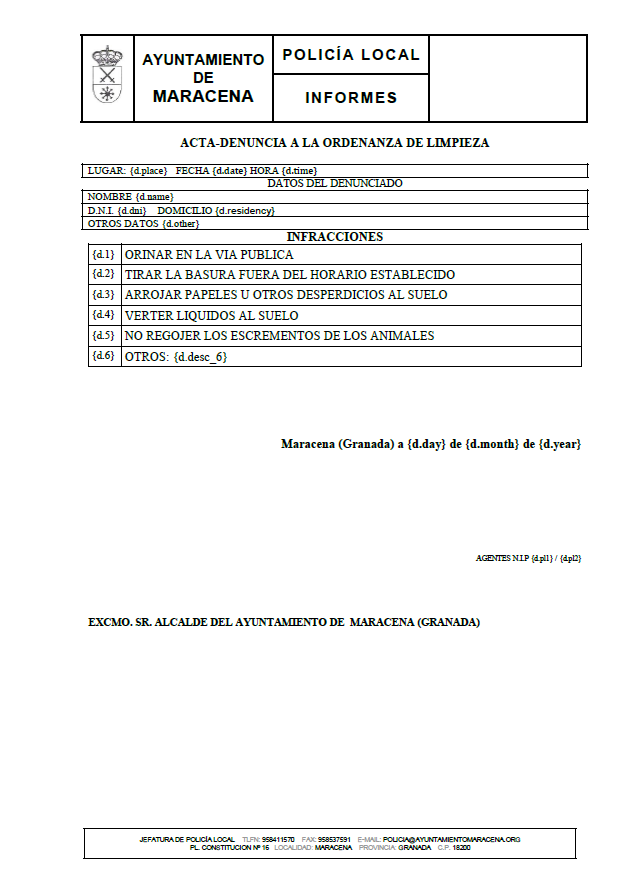
\includegraphics[scale=0.75]{imagenes/clean-template.png}
	\caption{Plantilla de ejemplo antes de ser rellena.}
\end{figure}

\begin{figure}[H]
	\centering
	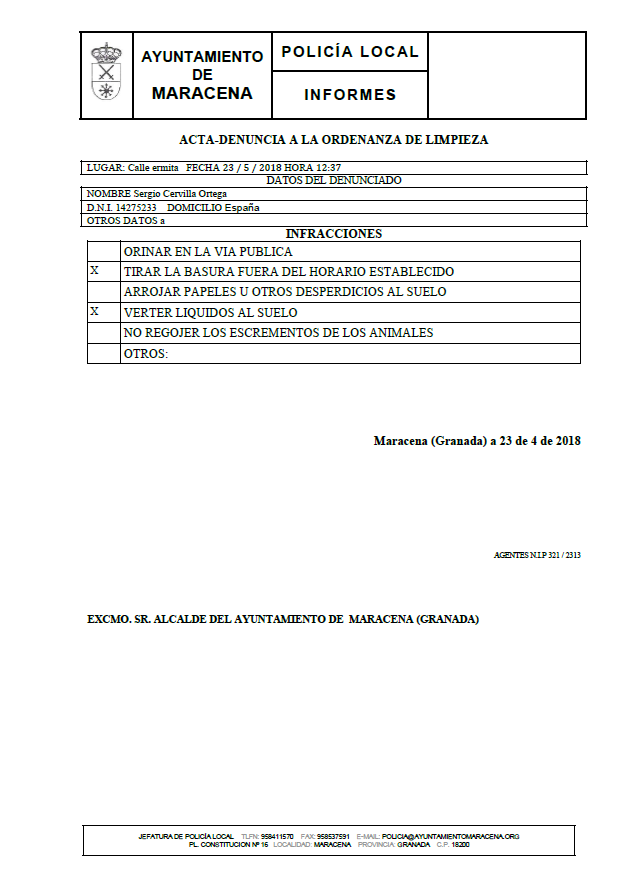
\includegraphics[scale=0.75]{imagenes/clean-res.png}
	\caption{Documento final.}
\end{figure}

\section{Desarrollo del sistema de croquis.}

En esta etapa del desarrollo el agente ya dispone de un sistema de acceso y de documentación completa. Para este hito se piensa en la dificultad que tiene un agente para 
demostrar que los hechos han ocurrido tal y como se han registrado pasado un tiempo del incidente.\\

Por ejemplo, hay un accidente porque el \textit{vehículo A} no ha respetado un ceda el paso e impacta contra el \textit{vehículo B} generando ciertos desperfectos en ambos
vehículos. Los involucrados junto con los agentes realizan un parte en el que quedan constatados los daños.  Un tiempo después, hay una reclamación por parte de uno de los
involucrados debido a que su vehículo tiene más desperfectos de los que se apuntaron a causa del accidente y el seguro no se hace responsable de cubrir dichos desperfectos
debido a que en el parte no se menciona nada acerca de dichos daños. En este caso, es su palabra contra la del agente.\\

Para evitar estas situaciones se ha diseñado este sistema. El agente podrá tomar varias fotografías de los hechos y dibujar sobre ellas todo lo que necesite. Además, se 
pueden hacer anotaciones sobre la propia imagen para reflejar datos de importancia como la dirección en la que venían los vehículos, resaltar puntos de la imagen...\\

Una vez el agente ha realizado todas las fotografías pertinentes y con todo lujo de detalles para que no pueda ocurrir la situación previamente descrita,
puede proceder a enviarlas al servidor donde quedarán almacenadas para posteriores consultas. De este modo, aunque pase mucho tiempo, siempre se podrá recurrir a 
las fotografías de aquel momento con todas las anotaciones que se tomaron para situarse en un contexto lo más cercano posible al de la incidencia. \\

Para desarrollar esta funcionalidad se ha utilizado \textit{canvas}\cite{canvas}. Este tipo de elemento es muy potente debido a que está expresamente diseñado para 
dibujar gráficos en un entorno web utilizando JavaScript. Cabe destacar, que \textit{canvas} es \textbf{únicamente} un elemento que está preparado para contener gráficos.
Es decir, los tenemos que insertar mediante el uso de JavaScript y no forman parte del elemento de forma nativa.\\

Para crear el croquis, el agente puede tomar una foto o subir una desde el almacenamiento interno. Una vez cargada la imagen, se mostrará en pantalla y se podrá 
dibujar sobre ella. Para lograr esta funcionalidad, se detecta cuando se ha subido una imagen a la aplicación y la inserta directamente en el canvas, sobre el que 
podremos dibujar y, además, borrar el contenido del croquis si es erróneo, o se quiere volver a comenzar.\\

Ejemplo de un croquis realizado en un accidente:

\begin{figure}[H]
	\centering
	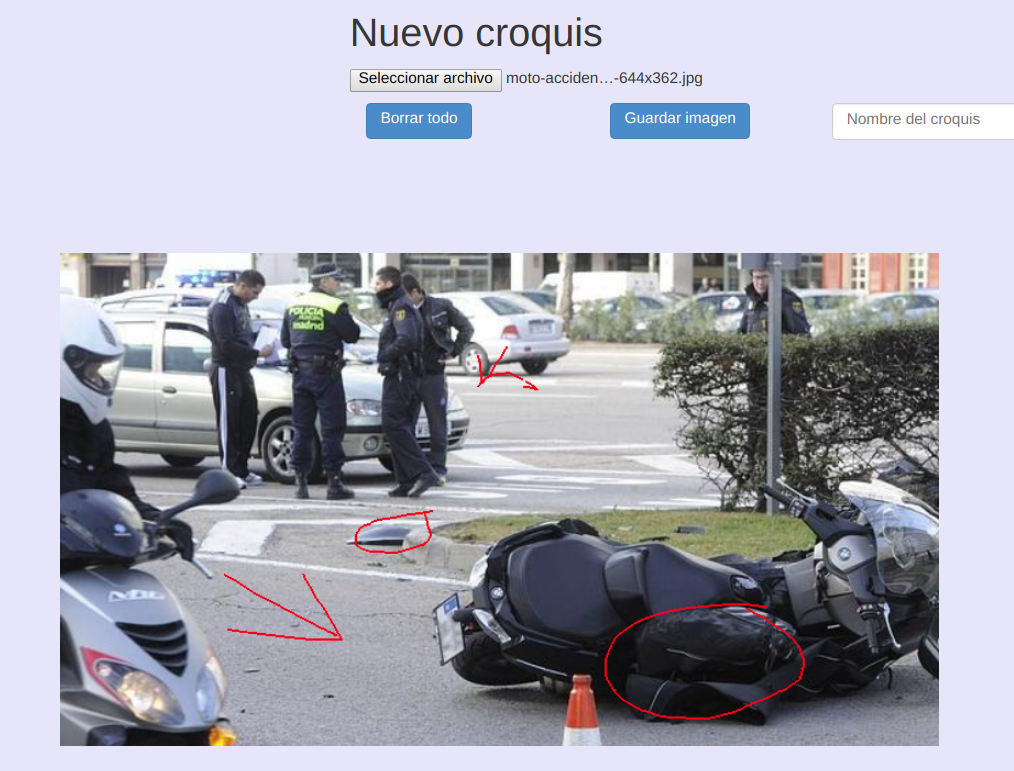
\includegraphics[scale=0.45]{imagenes/sketch.png}
	\caption{Uso del croquis en un accidente.}
\end{figure}


\section{Tests unitarios.}

En este hito ya se dan por realizadas las funcionalidades que podrán usar los agentes. En este punto, nos centramos en probar la calidad del software y del diseño.
Para ello, se ha empleado un sistema de \textbf{test unitarios}.\\

Los test unitarios están realizados con el propósito de probar las funcionalidades de la aplicación y así poder evitar los posibles errores en nuestro código \textbf{antes}
del despliegue de la aplicación. Estos tests se implementan de manera individual y el objetivo de cada uno de ellos es probar una funcionalidad. Para ello, se realizan varias
pruebas sobre la misma característica con distintas entradas y de las que conocemos los resultados que debieran ser correctos o erróneos. Un hecho relevante en la inclusión
de estos tests en nuestro sistema es que, además de garantizar el correcto funcionamiento de la aplicación antes de realizar el despliegue, es que pueden ser automatizados. 
De esta manera y con la ayuda de un sistema de integración continua que veremos en el siguiente punto, conseguimos que cada vez que se realice una modificación en nuestro software
se compruebe la integridad del sistema rehaciendo los tests.\\

\begin{figure}[H]
	\centering
	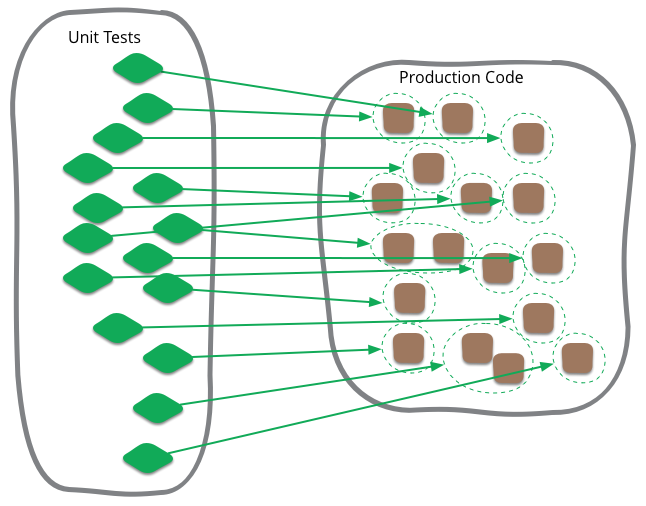
\includegraphics[scale=0.45]{imagenes/unit-test.png}
	\caption{Esquema del funcionamiento de los tests unitarios.\cite{image-unit-test}}
\end{figure}

En este caso, se ha utilizado la biblioteca \textit{supertest}\cite{supertest}, la cual nos proporciona un alto nivel de abstracción para probar nuestro servidor web.
Los test unitarios que se han realizado prueban las siguientes funcionalidades:

\begin{itemize}
	\item \textbf{Servidor.} Se realizan consultas a todas las rutas posibles de la aplicación para comprobar que todas existen y que además, solo se puede acceder 
	si se está previamente identificado. De este modo, garantizamos no solamente que todas las rutas posibles de la aplicación están operativas, sino que podemos garantizar
	que ningún usuario no identificado va a poder acceder a esta aplicación, consiguiendo probar parte de la seguridad de la aplicación antes del despliegue.
	\item \textbf{Base de datos.} Se realiza la creación de un usuario de prueba y se añade a la base de datos. Posteriormente, se comprueba si dicho usuario a quedado registrado
	en la base de datos y se procede a borrar para no ensuciar los registros. De igual manera se realiza con las incidencias, creando una de prueba y probando posteriormente que
	existe. Una vez realizado este test, se puede estar seguro de que la base de datos está configurada correctamente y completamente funcional.
\end{itemize}  

\section{Integración continua.}

Como objetivo de este hito, se propone añadir a nuestro desarrollo un sistema de integración continua.\\

La integración continua se creó con la intención de realizar el proceso de integración del software (ejecución de los tests) de la manera más habitual posible. De este modo, 
podemos detectar los fallos de manera inmediata y antes de que pase a la etapa de producción.\\

Para lograrlo se ha utilizado \textit{Travis CI}\cite{travis-ci}. Con esta herramienta es muy rápido y sencillo añadir la integración continua a nuestro repositorio. Para ello,
tan solo tenemos registrarnos en su página web con nuestra cuenta de GitHub y seleccionar el repositorio. Para que funcione correctamente, se debe crear un fichero de configuración
llamado \verb|.travis.yml|. Este archivo es el encargado de indicarle a \textit{Travis} el contexto en el que se ejecutarán los test, por tanto contiene
información relacionada con el lenguaje de programación utilizado, las versiones utilizadas, si se necesita permisos de superusuario...\\

En la siguiente imagen se representan los siguientes estados por los que pasa el código fuente desde que se añade hasta que ha pasado todos los test y la fase de integración.

\begin{figure}[H]
	\centering
	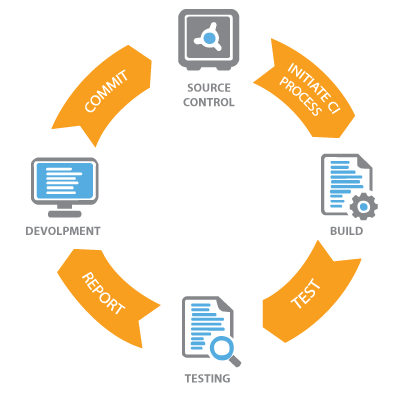
\includegraphics[scale=0.6]{imagenes/continuous-integration.png}
	\caption{Esquema del funcionamiento de un sistema de integración continua.\cite{image-ci} \label{fig:figura14}}
\end{figure}

\section{Instalación de la aplicación de manera automática.}
Para finalizar el desarrollo, se ha configurado el entorno de tal manera que la aplicación se configure automáticamente y esté lista para desplegarse de manera inmediata.\\

Para conseguir dichos objetivos, se han utilizado dos herramientas presentadas en el previo análisis: \textit{Vagrant} y \textit{Ansible}. 

\subsection{Creación del entorno.}

La aplicación se ejecutará bajo una máquina virtual que corre con \textit{Ubuntu 16.04}. La elección de este sistema operativo ha sido en base a los siguientes motivos:
\begin{itemize}
	\item \textbf{Compatibilidad.} Aunque la aplicación será compatible con todos los navegadores del mercado, el servidor deberá estar basado en Linux. Además, 
	Ubuntu en la versión 16.04 es LTS(\textit{Long Term Support}), por lo tanto, es una buena opción para mantener una máquina virtual a largo plazo. Otro motivo para
	elegir este sistema operativo en concreto y no su versión \textit{Server} es debido a que \textit{Vagrant} no tiene una imagen oficial de dicho sistema. Por tanto,
	para evitar vulnerabilidades a largo plazo se ha optado por esta versión en concreto.
	
	\item \textbf{Uso.} Ubuntu es la distribución basada en Linux más usada del mundo\cite{ubuntu-usage} y por tanto tiene una amplia comunidad de desarrolladores. Esto
	hace que sea un sistema operativo muy estable en sus versiones \textit{LTS}, lo cual es ideal para nuestro servidor.
\end{itemize}

Una vez elegido el sistema operativo, \textit{Vagrant} realiza las siguientes operaciones:

\begin{itemize}
	\item \textbf{Instala el S.O.} Si no hay registro en la máquina local del S.O, lo descargará e instalará antes de comenzar.
	\item \textbf{Actualiza el S.O.} Comprueba la versión del sistema operativo en busca de nuevas actualizaciones antes de lanzar la máquina virtual.
	\item \textbf{Ajusta las claves ssh.} Utiliza un esquema de llave pública/privada y de este modo podremos acceder a la máquina virtual de manera segura y sin contraseña.
	\item \textbf{Redirecciona los puertos.} Configura los puertos que queramos redireccionar de nuestra máquina local a la virtual, consiguiendo desviar el tráfico 
	para ser atendido por nuestro servidor.
	\item \textbf{Aprovisiona.} Ejecuta \textit{Ansible} para aprovisionar a la máquina con los recursos necesarios.
\end{itemize}

Una vez se llega a este punto, \textit{Vagrant} ejecuta el \textit{Playbook} de \textit{Ansible}. Dicho fichero contiene las instrucciones necesarias para 
preparar la máquina con todas las dependencias que tenga nuestro proyecto. Esto se traduce directamente en que con este tipo de ficheros se puede automatizar acciones
como actualizar la lista de paquetes del sistema, descargar dependencias globales de la aplicación, instalar \textbf{Chief}, ejecutar los test, lanzar la aplicación...\\



	% Presupuesto

	% Conclusiones
	\chapter{Conclusiones y trabajos futuros}

Este desarrollo se ha completado utilizando exclusivamente recursos libres, tanto la información consultada a lo largo del proyecto, como 
las herramientas y bibliotecas necesarias. De esta manera, se ha conseguido crear un software \textbf{completamente libre} que puede
ser usado para órganos del gobierno, como en este caso, un Ayuntamiento. \\

De igual manera que se ha completado satisfactoriamente el objetivo de ayudar a los agentes de policía. Aunque este desarrollo abarca hasta 
una fase temprana de la aplicación, los agentes han quedado muy satisfechos con el contenido que proporciona esta versión y en el entorno
de pruebas ha sido todo un éxito.\\

Por otro lado, se ha aprendido a gestionar un proyecto a gran escala desde 0. El desarrollo podría haber sido más rápido si no se hubieran 
incluido los \textit{test unitarios} o el \textit{despliegue y provisionamiento} pero la calidad del código hubiera disminuido. Incluyendo
esta metodología, podemos garantizar que nuestra aplicación ha sido probada ante un gran número de entradas, demostrando la robustez del sistema. 
De igual modo, la realización de un sistema de aprovisionamiento y despliegue garantiza la portabilidad y usabilidad. Esto se debe a que
un usuario no tiene que preocuparse de configurar el entorno, sino que directamente se crea y se configura de manera automática. Así, conseguimos
acortar el tiempo que se tarda en desplegar \textbf{Chief} tanto en local para realizar pruebas de desarrollo como en la nube para pasar el estado de
producción.\\

Sin duda alguna, se han podido probar los conocimientos adquiridos durante el transcurso del grado. Sin dichos conocimientos no hubiera sido
posible estructurar un proyecto de tales dimensiones. Tampoco se hubieran podido utilizar todas las tecnologías vanguardistas usadas durante 
el desarrollo ya que no se hubiera sido capaz de aprenderlas en un plazo tan limitado de tiempo.\\

Para futuros trabajos, sin duda alguna, se desplegaría la aplicación en un sistema en producción donde los agentes puedan utilizarlo en su día
a día. Además, se seguirían añadiendo nuevas funcionalidades como un sistema de localización en tiempo real, la posibilidad de gestionar los cuadrantes de los agentes e incorporar nuevos documentos para ayudar a los agentes a servir de una manera más efectiva a los ciudadanos.

	% Trabajos futuros


	
	\newpage
	\bibliography{bibliografia}
	\bibliographystyle{plain}
	
\end{document}

